% Level 3 workbook, Week 11 -- Project Studio 2
\chapterweek{11}{Project Studio 2}{Test it, playtest it, polish it, explain it.}

\section{What you will do}
\begin{itemize}[itemsep=1pt]
  \item Write at least \textbf{five pytest tests} for your own classes (Milestone 3).
  \item \textbf{Playtest} with a partner and sort the bugs you find (\textbf{triage}).
  \item Write a \textbf{README} and check your project is \textbf{accessible} (Milestone 4).
\end{itemize}

\section{Tests: crash-test dummies for your code}
A test is a tiny program that checks your program. Test the \textbf{logic} (moving, scoring, saving), not the drawing. Test \textbf{normal} cases and \textbf{edge} cases: the corner, the wall, the empty list, the last life.

\subsection{Example: tests for a tiny Player}
\begin{pycode}[muncher\_demo.py]
class Player:
    def __init__(self, row, col):
        self.row = row
        self.col = col
        self.score = 0

    def move(self, grid, d_row, d_col):
        new_row, new_col = self.row + d_row, self.col + d_col
        if grid[new_row][new_col] == "#":
            return False
        self.row, self.col = new_row, new_col
        if grid[new_row][new_col] == "*":
            self.score += 10
            grid[new_row][new_col] = "."
        return True
\end{pycode}
\begin{pycode}[test\_muncher\_demo.py]
from muncher_demo import Player

def make_grid():   # a tiny maze: wall, empty, star, empty, wall
    return [list("#####"), list("#.*.#"), list("#####")]

def test_player_moves_into_an_empty_cell():
    p = Player(1, 1)
    assert p.move(make_grid(), 0, 1) is True
    assert (p.row, p.col) == (1, 2)

def test_walls_block_the_player():          # edge case
    p = Player(1, 1)
    assert p.move(make_grid(), -1, 0) is False
    assert (p.row, p.col) == (1, 1)

def test_eating_a_star_scores_10_once():    # edge case
    grid = make_grid()
    p = Player(1, 1)
    p.move(grid, 0, 1)
    p.move(grid, 0, -1)
    p.move(grid, 0, 1)
    assert p.score == 10
\end{pycode}
\textbf{How to run your tests:} in Thonny choose \menu{Tools} $\rightarrow$ \menu{Open system shell...}, make sure you are in your project folder, and type \texttt{python -m pytest -q}. Each dot is a passing test; an \texttt{F} is a failing one, with its name and the line that failed.

\begin{tip}[Is my test any good?]
Break your code on purpose. Does the test go red? If not, the test is not checking anything. Then fix the code and watch it go green.
\end{tip}

\begin{exercise}[My five tests (Milestone 3)]
Plan your tests, then write them in \texttt{test\_<your project>.py}. At least one must be an edge case.
\begin{center}\small
\begin{tabular}{|p{0.5cm}|p{6.3cm}|p{5cm}|p{1.4cm}|}
\hline
\# & \textbf{Test name} (\texttt{test\_...}) & \textbf{What it checks} & \textbf{Edge?}\\ \hline
1 & & & \\[0.4cm] \hline
2 & & & \\[0.4cm] \hline
3 & & & \\[0.4cm] \hline
4 & & & \\[0.4cm] \hline
5 & & & \\[0.4cm] \hline
\end{tabular}
\end{center}
\end{exercise}

\section{Playtest and triage}
In a \textbf{playtest}, someone else uses your project while you watch \textbf{silently} and take notes. Every time they get stuck, you learn something. Afterwards, sort the notes into three piles -- that is called \textbf{triage}:
\begin{center}
\begin{tikzpicture}[pile/.style={draw,thick,rounded corners=3pt,minimum width=4.2cm,minimum height=1.4cm,align=center,font=\small}]
  \node[pile,fill=kcvermillion!20] at (0,0) {\textbf{1 Must fix}\\crashes, cannot start,\\cannot win};
  \node[pile,fill=kcorange!20] at (4.6,0) {\textbf{2 Should fix}\\confusing, unfair,\\hard to read};
  \node[pile,fill=kcsky!20] at (9.2,0) {\textbf{3 Nice to have}\\new ideas for\\version 2};
\end{tikzpicture}
\end{center}
For a crash: first write a test that shows the bug, then fix it. The test makes sure it never comes back.

\begin{exercise}[Playtest feedback cards]
Cut these out (or copy them onto index cards). Fill in one card for each thing you notice while your partner plays.
\begin{center}
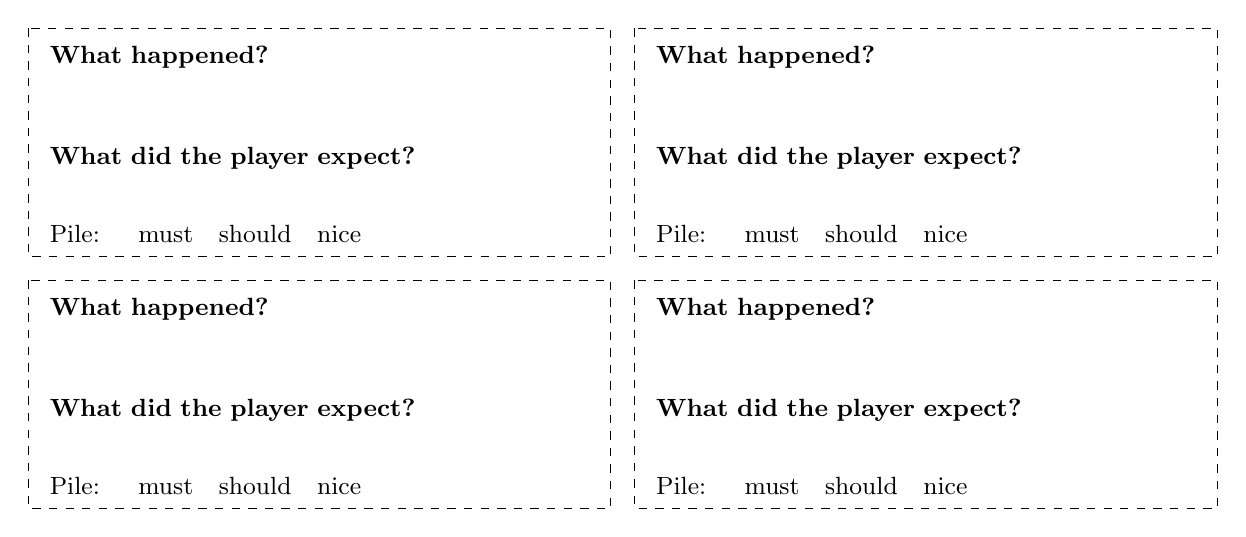
\begin{tikzpicture}
  \foreach \x/\y in {0/0,7.7/0,0/-3.2,7.7/-3.2}{
    \draw[dashed] (\x,\y) rectangle ++(7.4,-2.9);
    \node[anchor=north west,font=\small,text width=7cm] at (\x+0.15,\y-0.1) {\textbf{What happened?}\\[0.9cm]\textbf{What did the player expect?}\\[0.6cm]Pile: \ \ $\square$ must \ $\square$ should \ $\square$ nice};
  }
\end{tikzpicture}
\end{center}
\end{exercise}

\section{README: explain it to a stranger}
A README is the first thing people read. Future-you is a stranger too!

\begin{exercise}[My README (Milestone 4)]
Create \texttt{README.md} in your project folder with these sections:
\begin{checklist}
  \item \textbf{Title and one sentence}: what it is.
  \item \textbf{How to run it}: which file to open and press Run.
  \item \textbf{Controls}: keys or clicks.
  \item \textbf{How it works}: my classes (is-a / has-a), my data structure, my algorithm, the file it saves.
  \item \textbf{Tests}: how to run them, how many there are.
  \item \textbf{Credits}: my name as a nickname, and every borrowed thing with its licence (or \enquote{everything made by me}).
\end{checklist}
\end{exercise}

\begin{exercise}[Accessibility and usability check]
\begin{checklist}
  \item Colours come from the Okabe--Ito palette, and nothing depends on colour alone (shapes, letters or text too).
  \item Text is big enough to read from a chair.
  \item The controls are written on the screen.
  \item Nothing flashes fast.
  \item A new player knows what to do within 10 seconds.
  \item One thing I fixed today: \rule{6.5cm}{0.4pt}
\end{checklist}
\end{exercise}

\begin{vocab}
  \vocabword{edge case}{An unusual input at the limits: a corner, an empty list, zero, the last life.}
  \vocabword{playtest}{Watching someone use your project to find problems.}
  \vocabword{triage}{Sorting problems by how much they matter, to fix the important ones first.}
  \vocabword{README}{A file that explains what a project is, how to run it and how it works.}
  \vocabword{usability}{How easy something is to use for someone new.}
  \vocabword{accessibility}{Designing so that people with different abilities can use it too.}
\end{vocab}

\begin{reflection}
What did your playtester do that surprised you? \answerlines{1}
Which test are you proudest of, and why? \answerlines{1}
\end{reflection}
